\documentclass[letterpaper,12pt]{book}
\usepackage[utf8]{inputenc}
\usepackage[spanish]{babel}
\usepackage{amsmath}
\usepackage{amssymb}
%\usepackage{hyperref} \url de ogle
\usepackage{graphicx}
\usepackage{appendix}
\usepackage{adjustbox}
\usepackage{caption}
\usepackage{subcaption}
\DeclareMathOperator*{\argmax}{arg\,max}

\title{Clasificación de Series de Tiempo Astronómicas}
\author{Muriel Pérez\\ 201011755}
\begin{document}
\maketitle
\tableofcontents 
\chapter{Introducción}

Con los avances en técnicas de observación astronómica que han sucedido en los últimos años, hay grandes cantidades de datos disponibles. Por ejemplo se espera que el \textit{VISTA Variables in the Via Lactea} (VVV) del \textit{European Southern Observatory} (ESO) produzca del orden de $10^{9}$ curvas de luz\footnote{\label{nota:curvasDeLuz} La curva de luz de una estrella es el resultado de medir su magnitud como función del tiempo. La magnitud de una estrella es el flujo de energía observado en una parte del espectro electromagnético (una banda), delimitada por un filtro, en escala logarítmica (ver el capítulo 4 de \cite{karttunen_fundamental_2007}).} de fuentes puntuales en el infrarojo cercano con hasta 100 observaciones en diferentes épocas de alta calidad. De la misma forma estudios como la misión Kepler de la \textit{National Aeronautics and Space Administration} (NASA), cuyo objetivo principal es la detección de exoplanetas,  tienen como subproductos gran cantidad de curvas  de luz. 

Para que estos datos sean útiles para la comunidad científica es necesario clasificarlos y extraer sus características. Aunque los métodos automáticos muchas veces no pueden igualar la inspección manual por parte de un experto, la cantidad de datos disponible hace que esta tarea no sea posible en corto tiempo y hace necesario utilizar técnicas de minería de datos. Este interés se manifiesta en proyectos como el \textit{VVV Templates Project} que tiene como objetivo consolidar una base bien definida de curvas de luz de estrellas variables en el infrarojo cercano para ser utilzadas como referencia para la clasificación automática de curvas de luz.

Las curvas de luz no pueden ser analizadas con técnicas de análisis de series de tiempo porque, debido a limitaciones en el tiempo de observación, fallas técnicas, periodos de mantenimiento de los instrumentos utilizados y la imposibilidad de abservar todas las regiones del cielo durante todo el año, las curvas de luz no constan del mismo número de observaciones y éstas no son hechas en intervalos regulares por lo que el tiempo durante el cual cada estrella no es observada es impredecible y algunas características importantes de las curvas de luz no son observadas. 

Dependiendo de la serie de magnitudes observadas, una estrella puede ser clasificadas como variable o no variable; periódicas o no periódicas; y en diferentes clases de variabilidad estelar que depende de la morfología de su curva de luz. La forma de la curva de luz depende de las condiciones físicas de la estrella por lo que conocer a qué tipo de variabilidad pertenece cada estrella es de vital importancia para el estudio de las estrellas variables. A su vez, el estudio de las estrellas variables ha sido importante para el estudio de la evolución estelar, la determinación de distancias cósmicas y la búsqueda de exoplanetas, entre otras. 

En estudios previos \cite{debosscher_automated_2007, sarro_automated_2009, richards_machine-learned_2011} se le ha asignado a cada curva de luz un vector, llamado vector de características, y, basado en él, se ha hecho la clasificación automática. Este proceso consiste en entrenar un clasificador basado en una muestra clasificada previamente, la  muestra de entrenamiento, utilizando el vector de características escogido. La escogencia de el vector de características es crucial para el proceso de clasificación porque con él se debe poder clasificar cada curva de luz, es decir, debe logar que, en el espacio de características, las clases se superpongan lo menos posible. Para la conformación de este vector se han elegido coeficientes de Fourier de la curva de luz\cite{debosscher_automated_2007, sarro_automated_2009, richards_machine-learned_2011}, que son calculados mediante métodos como el periodograma de  Lomb-Scargle \cite{scargle_studies_1982} o la minimización de la entropía de Shannon de la gráfica de la curva \cite{cincotta_astronomical_1995}. 

Esta elección de caracterísicas no es del todo conveniente porque requiere de gran poder computacional y limita el tipo de objetos que pueden ser clasificados. El cálculo del periodogramas como el de Lomb-Scargle para curvas de luz, y en general el de los métodos utilizados en la literatura, requiere de intentar una gran cantidad de periodos candidatos a ser el periodo de la curva de luz para luego elegir el mejor y de la inspección manual de las curvas de luz. Los periodos de los objetos observados varía entre desde unos pocos minutos y varios años por lo cual se requiere probar una gran cantidad de periodos. Por un lado este es un proceso es computacionalmente intensivo, lo que limita su uso en conjuntos grandes de curvas de luz; y por otro lado no es seguro que dé como resultado el periodo real de una curva de luz, por lo que a menudo éste debe ser revisado manualmente. Además el resultado de la clasificación puede ser sensible a la calidad de las curvas de luz que sean elegidas como muestra de entrenamiento \cite{debosscher_automated_2007} y limita el estudio a fuentes periódicas.  

En \cite{rodriguez_feliciano_alisis_2012, sabogal_search_2014}, los autores notaron que algunas variables descriptivas de la serie de magnitudes de una curva de luz (como su sesgo o su curtosis) sirven para clasificar ciertos tipos de estrellas con clasificadores lineales. En este trabajo retomamos esa idea y construimos un vector de características basadas en variables tomadas de estadística descriptiva. El uso de este tipo de variables tiene las ventajas de que puede ser calculadas de manera rápida y da como resultado un vector de caracterísicas que sive para realizar clasificación con una taza de éxito alta. Para evaluar esta aproximación al problema utilizamos una parte del Catálogo de Estrellas Variables de la tercera fase del \textit{Optical Gravitational Lensing Experiment} (OGLE III)\cite{soszynski_optical_2011-2,soszynski_optical_2010,soszynski_optical_2009-1,soszynski_optical_2011,soszynski_optical_2010-2,soszynski_optical_2008-1,soszynski_optical_2013-1,soszynski_optical_2011-1,soszynski_optical_2009,pawlak_eclipsing_2013,graczyk_optical_2011,poleski_optical_2010,soszynski_optical_2013,soszynski_optical_2010-1,soszynski_optical_2008} que contiene curvas de luz  de estrellas previamente clasificadas en seis tipos de variabilidad estelar y curvas de luz de estrellas candidatas a ser clasificadas como Be (ver cuadro \ref{cuadro:datosUsados}).

En este trabajo utilizamos k-vecinos más cercanos, árboles de clasificación, máquinas de soporte vectorial y bosques aleatorios para realizar la clasificación automática de las curvas de luz basada en nuestra elección de características. Asímismo, estimamos la probabilidad de que una nueva curva de luz sea clasificada correctamente por uno de estos clasificadores utilzando validación cruzada de 10 iteraciones.  Estos clasificadores fueron elegidos porque son aproximaciones muy distintas al problema de clasificación, por su naturaleza no lineal y no paramétrica; y por el hecho de que han mostrado ser efectivos en gran cantidad de aplicaciones prácticas. Para todo el análisis utilzamos el paquete estadístico de fuente abierta $R$ (cita de R). Para cada tarea utilizamos paquetes específicos que son referenciados a lo largo del documento. 

%%Reescribir, así ya no está organizado el documento
Este documento está organizado de la siguiente forma. En el capítulo \ref{cap:losDatos} damos una descripción del conjunto de datos utilizado en este trabajo. En el capítulo \ref{cap:clasificacion} abordamos el problema de clasificación de manera informal, presentamos y discutimos la elección de atributos y evaluamos el desempeño de los clasificadores mediante validación cruzada de 10 iteraciones. En los apéndices abordamos formalmente el problema de aprendizaje en general y damos una descripción de cada uno de los algorítmos utilizados en el trabajo.

\chapter{El Problema del Aprendizaje}

Aquí diré cómo está organizado el capítulo.

\section{Lulu}

Las personas reconocemos con facilidad las letras en manuscritos, las caras de otras personas, las palabras que alguien nos dice o el estado de la comida basado en su olor. La capacidad de agrupar los estímulos que recibimos en categorías, por ejemplo el olor de la comida en buen o mal estado,y la capacidad para actuar en respuesta a ellos ha sido de vital importancia para nuestra supervivencia . Por ello  hemos desarrollado complejos sistemas para llevar a cabo estas tareas. 

Con la popularización de computadores electrónicos, la construcción máquinas que aprendan de la experiencia ha sido objeto de estudio. La habilidad de crear estas máquinas tiene una importancia estratégica puesto que existen tareas que no pueden ser llevadas a cabo utilizando técnicas de porgramación clásicas porque no existe un modelo matemático para ellas. En el caso de la clasificaciónd ecurvas de luz, por la forma en que se hacen las observaciones y el hecho de que la identificación de una curva de luz se hace con base en su forma, es difícil hacer un modelo matemático que capture estas diferencias. A pesar de esto existe gran gantidad de ejemplos de curvas de luz disponibles, por lo que es natural preguntarse si se puede entrenar un computador para identificar estas diferencias de la misma forma en que una persona puede ser entrenada para reconocerlas. En la figura \ref{fig:dosCurvas} se observan dos curvas de luz, una pulsante y una eruptiva, que pueden ser distinguidas utilizando únicamente esta información. La pregunta de si es posible entrenar un sistema basado en datos disponibles puede ser hecha para otras tareas, como el reconocimiento de textos en manuscritos, la detección e identificación de caras y objetos en imágenes o la identificación de genes en secuencias de ADN. 

\begin{figure}
  \centering
  \begin{subfigure}[b]{0.5\textwidth}
    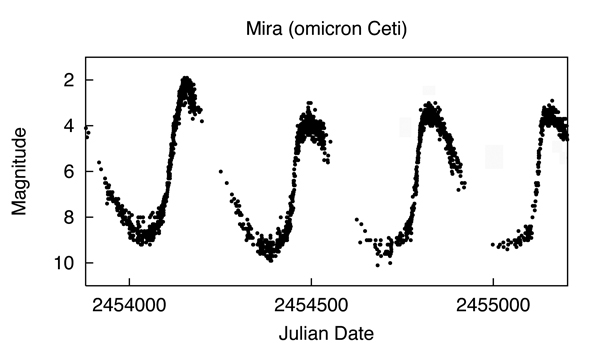
\includegraphics[width=\textwidth]{./img/CProblema/omicet.jpg}
    \caption{Curva de luz de una estrella Mira}
    \label{fig:gull}
  \end{subfigure}%
  ~ %add desired spacing between images, e. g. ~, \quad, \qquad, \hfill etc.
  % (or a blank line to force the subfigure onto a new line)
  \begin{subfigure}[b]{0.5\textwidth}
    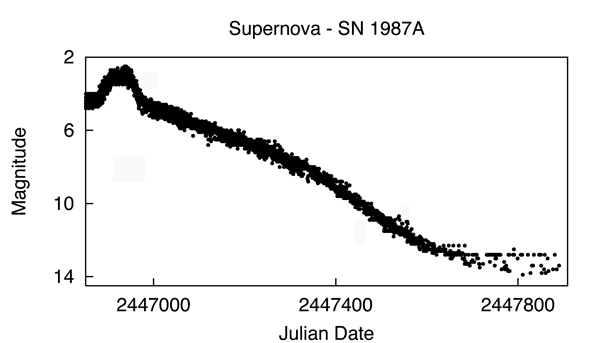
\includegraphics[width=\textwidth]{./img/CProblema/sn1987a.jpg}
    \caption{Curva de luz de la Supernova 1987A}
    \label{fig:tiger}
  \end{subfigure}
  ~ %add desired spacing between images, e. g. ~, \quad, \qquad, \hfill etc.
  % (or a blank line to force the subfigure onto a new line)
  \caption{Las estrellas pueden ser clasificadas en grupos basado en la forma de sus curvas de luz. Estas clasificación puede ser hecha con base en la forma de las curvas de luz, sin embargo es difícil crear un modelo matemático que capture estas diferencias. Imágenes tomadas de \cite{bsj_types_2012}}\label{fig:dosCurvas}
\end{figure} 

El reconocimiento de patrones es una disciplina científica cuya meta es la clasificación de objetos en clases. Existen situaciones en las cuales existe una gran cantidad de objetos previamente clasificados en clases predefinidas y la tarea es encontrar, o aproximar lo mejor posible, la dependencia funcional entre objetos y clases. Podemos precisar esto de la siguiente forma. Llamemos al espacio de los objetos que queremos clasificar $X$y $\{1,\dots, M\}$ es el conjunto de las posibles clases a las que pueden pertenecer los elementosd e $X$.  En el caso de la clasificación de curvas de luz, $X$ consta de todas las curvas de luz y  $\{1,\dots, M\}$ representa los posibles tipos de variabilidad estelar. Contamos con una muestra aleatoria, llamada muestra de entrenamiento, $\mathcal{L} = \{(x_i,j_i), \dots, (x_N,j_N)\}$  con $x_l\in X$ y $j_l\in \{1, \dots, M\}$, es decir, una muestra de $X$ previamente clasificada. Nuestra tarea es entonces proponer una función $g:X\rightarrow \{1,\dots, M\}$ a partir de la información contenida en $\mathcal{L}$, que representa nuestra predicción de la clase a la que pertenece cada elemento de $X$. La función $g$ se llama clasificador y, para un elemento $x\in X$ cuya clase $j$ es desconocida, el clasificador falla si $g(x)\neq j$.

El espacio $X$ puede ser complejo o no estar matemáticamente bien definido, por lo cual con frecuencia se representan los objetos con vectores, llamados de características,  en $\mathbb{R}^n$. Por ejemplo si queremos realizar detección de rostros, $X$ consiste de todos los posibles rostros, por lo que es más conveniente representar cada rostro con un conjunto de números como la separación de los ojos, el ángulo que forma las líneas que unen los ojos con la barbilla, etcétera; lo mismo sucede con las curvas de luz, por lo que representamos cada una con un vector. Estos vectores de características pueden, en principio, ser una combinación de variables continuas, discretas y categóricas, sin embargo esto no afecta en gran medida la teoría. Así las cosas, la elección de un clasificador puede ser una función $g:\mathbb{R}^n\rightarrow \{1, \dots, M\}$.

Se debe utilizar un marco probabilístico para modelar la dependencia entre características y clases. Puede suceder que dos observaciones con un mismo vector de características pertenezcan a clases diferentes. Esto puede suceder en escenarios en los que pertenencia a una u otra clase no so sea completamente explicada por diferencias en los vectores de características, o porque la dependencia real entre características y clases sea no determinista. En este orden de ideas suponemos que existe una medida de probabilidad $P$ sobre $\mathbb{R}^n\times \{1, \dots, M\}$ tal que $P(\vec{x}, j)$ es la probabilidad de observar un vector de características $\vec{x}\in\mathbb{R}^n$ cuyo objeto representado pertenece a clase $j$. Así definimos la probabilidad de error del clasificador $g$, $P_{e}(g)$, como 
\begin{equation}
P_e(g) = P(g(\vec{x})\neq j).
\end{equation}

Surge entonces la pregunta de qué tan bueno puede ser un clasificador. El mejor clasificador posible es llamado el clasificador de Bayes.

\section{El Clasificador de Bayes}

Decimos que un clasificador $g_B:\mathbb{R}^n\rightarrow \{1, \dots, M\}$ es de Bayes si minimiza la probabilidad de error, es decir, que si $g$ es otro clasificador entonces
\begin{equation}
P_e(g_B) \leq P_e(g).
\end{equation}
Llamaremos $P_{e}^{*}$ a  $P_e(g_B)$.

En el caso de que existan densidades condicionales $f_j$ tales que para cada $A\subset \mathbb{R}^n$ medible se cumple
\begin{equation}
P(A|j) =\int_{A}f_{j}(\vec{x})d\vec{x}
\end{equation}
podemos dar una expresión explícita para el clasificador de Bayes. Para un clasificador $g$ podemos escribir
\begin{equation}
  \begin{aligned}
    P_e(g) &= 1-P(g(\vec{x}) =  j)\\
    & = 1-\sum_{j=1}^{M} P(g(\vec{x}) = j|j)P(j)\\
    & = 1-\sum_{j=1}^{M}\left( \int_{\{g(\vec{x})=j\}}f_j(\vec{x})  d\vec{x} \right) P(j)\\
    & = 1 - \int \sum_{j=1}^{M} \chi_{\{g(\vec{x})=j\}}f_j(\vec{x})P(j)d\vec{x}.
  \end{aligned}
\end{equation}
Donde $P(j)$ es la probabilidad \textit{a priori} de encontrar un objeto de clase $j$. Ahora, para cada $\vec{x}$ 
\begin{equation}\label{eq:bayesIneq}
\sum_{j=1}^{M}\chi_{\{g(\vec{x})=j\}}f_j(\vec{x})P(j) \leq \max_j[f_j(\vec{x})P(j)]
\end{equation}
entonces
\begin{equation}\label{eq:bayesIneq}
P_e(g)\geq \int \max_j[f_j(\vec{x})P(j)] d\vec{x}.
\end{equation}
Como la desigualdad \ref{eq:bayesIneq} es igualdad cuando $g$ le asigna a cada $\vec{x}$ la clase $j$ para la cual $f_j(\vec{x})P(j)$, podemos concluir que éste es el clasificador de Bayes, es decir,
\begin{equation}
  g_B(\vec{x}) = \argmax_{j\in\{1,\dots,M\}}f_j(\vec{x})P(j)
\end{equation}
y
\begin{equation}
  P_e^* = \int \max_j[f_j(\vec{x})P(j)] d\vec{x}.
\end{equation}


\section{Clasificadores}

\subsection{K Vecinos Más Cercanos}

\subsection{Máquinas de Soporte Vectorial}

\subsection{Árboles de Clasificación y Regresión}

\subsection{Bosques Aleatorios}


\chapter{El conjunto de Datos\label{cap:losDatos}}

Los datos utilizados en este trabajo provienen de la tercera fase del \textit{Optical Gravitational Lensing Experiment} (OGLE-III). OGLE es un proyecto de larga duración cuyo objetivo principal es la búsqueda de materia oscura mediante el aprovechamiento de lentes gravitacionales. La tercera fase del protecto comenzó en 2001 y hace uso de un telescopio de $1.3$m de diámetro localizado en el observatorio de Las Campanas, Chile\cite{udalski_optical_2004}. Uno de los principales resultados de OGLE-III es la reducción y publicación \cite{udalski_optical_2008} de las curvas de luz de objetos en el bulbo de la Galaxia, la Gran Nube de Magallanes y la Pequeña Nube de Magallanes. En este trabajo utilizamos las curvas de luz de $431 653$ objetos del catálogo de estrellas variables de OGLE-III de seis tipos de variabilidad (ver tabla \ref{cuadro:datosUsados}) al cual se puede acceder en la página del proyecto \footnote{http://ogle.astrouw.edu.pl/} y $475$ curvas de luz de estrellas candidatas a ser clasificadas como Be (ESCRIBIR DE DÓNDE FUERON TOMADAS ESTAS).

Las curvas de luz tomadas del catálogo de estrellas variables de OGLE-III se encuentran clasificadas por tipo de variabilidad estelar en un proceso que que involucró, en una etapa, la inspección manual de las curvas de luz (ver referencias en la tabla \ref{cuadro:datosUsados}) por lo cual tomaremos esta clasificación como verdadera. En este trabajo utilizamos únicamente las curvas de luz registradas en la banda I \footnote{Los objetos observados emiten radiación en una parte amplia del espectro electromagnético. Los telescopios utilizan filtros para recoger solo la radiación emitida por estos objetos en ciertas partes del espectro electromagnético. El filtro I (infrarojo) tiene un ancho de banda de 149nm y una longitud de onda efectiva de 797nm (ver \cite{karttunen_fundamental_2007})} a pesar de que también se encuentra disponible información adicional sobre las curvas de luz como sus periodos y algunos coeficientes de Fourier (ver referencias en la tabla \ref{cuadro:datosUsados}). Esta elección se debe a que el cálculo de estas cantidades es computacionalmente intensivo, no siempre se encuentran disponible y proponemos hacer la clasificación utilizando variables tomadas de estadística descriptiva.

\begin{table}
  \centering  
  \begin{tabular}{rr}
    \hline
    \hline
    Tipo de variabilidad y origen & \shortstack{Número \\de Objetos}\\
    \hline
    \hline 
    RR Lyrae - BG\cite{soszynski_optical_2011-2} & 16836\\
    RR Lyrae - PNM \cite{soszynski_optical_2010}& 2475\\
    RR Lyrae - GNM \cite{soszynski_optical_2009-1}& 24906\\
    \hline
    Cefeidas - BG \cite{soszynski_optical_2011}& 32\\%El título del paper es classical and type2 cepheids
    Cefeidas - PNM \cite{soszynski_optical_2010-2}& 4630\\
    Cefeidas - GNM \cite{soszynski_optical_2008-1}& 3361\\
    \hline
    Variables de Largo Periodo - BG \cite{soszynski_optical_2013-1}& 232406\\
    Variables de Largo Periodo - PNM \cite{soszynski_optical_2011-1}& 19384\\
    Variables de Largo Periodo - GNM \cite{soszynski_optical_2009}& 91995\\
    \hline
    Sistema Binario Eclipsante - PNM \cite{pawlak_eclipsing_2013}& 6138\\
    Sistema Binario Eclipsante - GNM \cite{graczyk_optical_2011}& 26121\\
    \hline
    $\delta$-Scuti - Nube Mayor de Magallanes\cite{poleski_optical_2010} & 2786\\
    \hline
    Cefeidas Tipo II - BG \cite{soszynski_optical_2013}& 335\\
    Cefeidas Tipo II - PNM \cite{soszynski_optical_2010-1}& 43\\
    Cefeidas Tiplo II - GNM \cite{soszynski_optical_2008}& 197\\
    \hline
    Cadidata a Be -  Vía Láctea (cita!) & 475\\
    \hline
    \hline 
  \end{tabular} 
  \caption{Conjunto de datos utilizados. BG hace referencia al Bulbo Galáctico; PNM, a la Pequeña Nube de Magallanes y GNM, a la Gran Nube de Magallanes. }
  \label{cuadro:datosUsados}
\end{table}


Agrupamos los $432128$ objetos disponibles en siete clases de variabilidad estelar (ver tabla\ref{cuadro:cantidadDatos}). Esta elección de clases puede ser refinada puesto que en cada una de estas clases existen subclases. Por ejemplo entre las Cefeidas se puede distinguir entre aquellas que pulsan en su modo fundamental, en su primer sobretono (segundo armónico) o en su segundo sobretono (tercer armónico)  (ver figura \ref{fig:tiposCefeidas}). Sin embargo conocer a qué clase de variabilidad estelar pertence un objeto facilita considerablemente su clasificación en subclases y análisis subsecuentes. 

\begin{table}[ht]
  \centering
  \begin{tabular}{rrr}
    \hline
    Tipo de Variabilidad & Cantidad \\
    \hline
    Variables de Largo Periodo (VLP) & 343782 \\
    RR Lyrae (RRLyr) & 44217\\
    Cefeida (Cef)& 8004\\
    Sistema Binario Eclipsante (SBE)&32259 \\
    $\delta$-Scuti ($\delta$Sct)& 2788\\
    Cefeida Tipo II (CefT2)& 603\\
    Candidata a Be (BeEC)& 475\\
    \hline
    Total & 432128\\
    \hline
  \end{tabular}
  \caption{Cantidad de datos por tipo de variabilidad}
  \label{cuadro:cantidadDatos}
\end{table}




\begin{figure}
  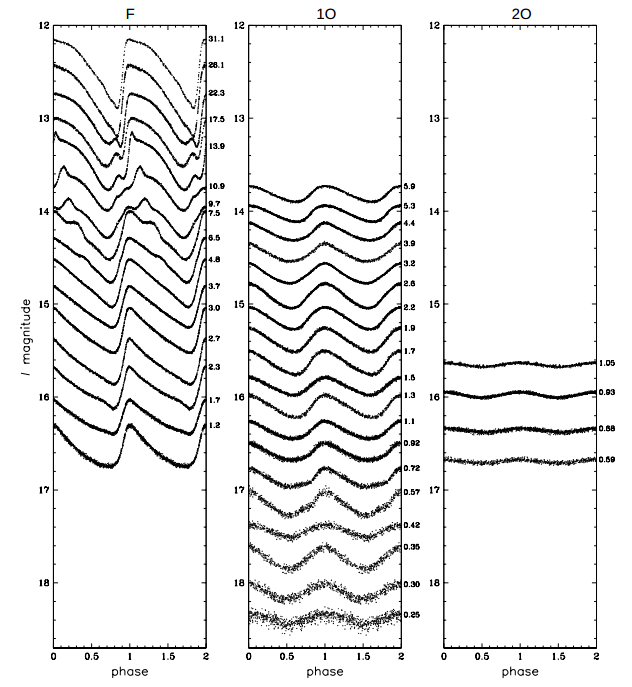
\includegraphics[width = \textwidth]{./img/C2Datos/tiposCefeidas.png}
  \label{fig:tiposCefeidas}
  \caption{Curvas de luz ilustrativas de Cefeidas en modo fundamental (izquierda), primer sobretono (mitad), segundo sobretono (derecha). Los números pequeños a la derecha de cada recuadro muestran los periodos redondeados de las curvas de luz presentadas en los recuadros. Tomado de \cite{soszynski_optical_2011}}
\end{figure}

En el Catálogo de Estrellas Variables de OGLE-III, cada curva de luz está disponible en un archivo que contiene tres columnas con los valores de magnitud, fecha juliana \footnote{La fecha Juliana es el tiempo medido en días desde el 1 de enero de 4713 a. C.} en la que fue tomada cada medida y error en la medida de la magnitud. El número de medidas para cada objeto y la separación temporal varía ampliamente. La separación mínima dos mediciones en toda la muestra es de 0.00147d, la máxima es 2156.9d y en promedio están separadas por 5.1d; por su parte el número promedio de observaciones por objeto es 759; el máximo, 5173; y el mínimo,  11. El 75\% de los objetos cuenta con más de 386 observaciones. Para todos los objetos estas observaciones están repartidas en los (número de años) años en que estuvo activo OGLE-III. En la figura \ref{fig:curvaDeLuz} se puede observar una curva de luz del catálogo de estrellas variables de OGLE-III.    

\begin{figure}
  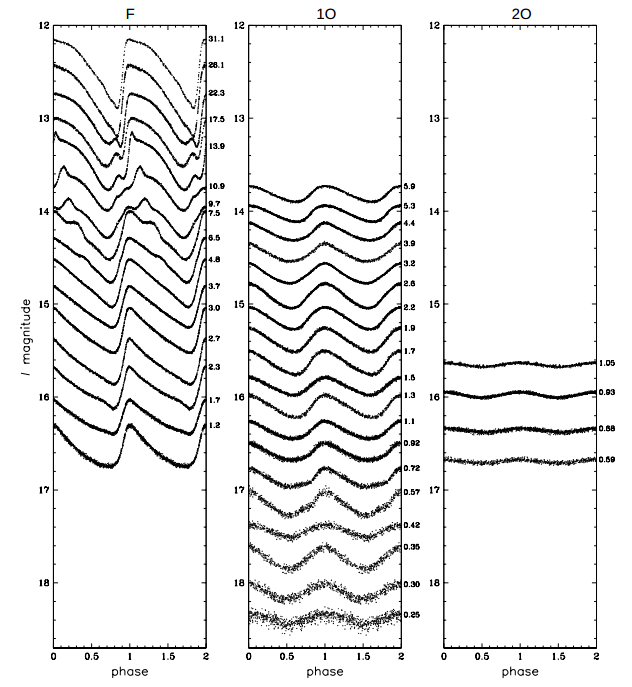
\includegraphics[width = \textwidth]{./img/C2Datos/tiposCefeidas.png}
  \label{fig:curvaDeLuz}
  \caption{(figura pendiente de imagen) Curva de luz (nombre del archivo) del catálogo OGLE-III. Los periodos en los que no hay mediciones corresponden a los momentos del año en los que la zona en la que se encuentra el objeto no puede ser observada debido a la posición relativa entre el Sol y la Tierra.}
\end{figure}

\chapter{Clasificación}\label{cap:clasificacion} 

Conociendo la curva de luz de un objeto podemos clasificarlo según su tipo de variabilidad estelar, sin embargo, esta relación no puede ser programada en un computador de manera sencilla. Cuando decimos que a cada curva de luz le corresponde un tipo de variabilidad estelar, queremos decir que existe una función, llamada función objetivo, cuya entrada es una curva de luz y cuya salida es un tipo de variabilidad estelar. El objetivo general del aprendizaje supervidado es aproximar esta función utilizando la experiencia previa. Esta experiencia previa es, en este caso, nuestro conjunto de datos (ver cuadro \ref{cuadro:datosUsados}) y la estimación de esta regla, o función de decisión, es encontrada mediante un algorítmo de aprendizaje. Un algorítmo de aprendizaje escoge una función de decisión de un conjunto de funciones, llamado conjunto de hipótesis, utilizando un criterio que usualmente consiste en la minimización de una función de costo asociada a las clasificaciones erróneas. En nuestro caso utilizamos como función de costo la probabilidad de clasificación incorrecta.

Cada curva de luz en nuestra muestra es una tríada que consta de una sucesión de mediciones de magnitud, una suseción de fechas y un tipo de variabilidad estelar. Como cada curva de luz tiene un número de mediciones diferentes que están repartidas en diferentes intervalos de tiempo, esto dificulta la implementación de algorítmos para entrenar una regla de desisión. En consecuencia, a cada curva de luz le asignamos un vector de dimensionalidad fija, llamado vector de características. Este vector puede ser, en principio, una combinación de variables categóricas y numéricas; en este trabajo le asignamos únicamente variables numéricas. La función de decisión divide el espacio de caracterísitcas en regiones tales que a cada elemento del espacio de características le asigna un tipo de variabilidad estelar basado en qué región se encuentra. Así, para clasificar una curva cuyo tipo de variabilidad es desconicido, calculamos su vector de caracterísicas y le asignamos la clase de variabilidad dada por la regla de decisión previamente entrenada. Por lo tanto la elección de características es crucial puesto que si los vectores de características de diferentes clases se superponen, no podrán ser distinguidos por la regla de decisión.

Subsecuentemente llamaremos $g:\mathbb{R}^{n}\rightarrow \{VLP,\dots, BeEC\}$ a la función de decisión en cuestión que le asigna a cada vector de características un tipo de variabilidad (ver cuadro \ref{cuadro:cantidadDatos}). Cada dato es representado por una pareja $(\vec{x}, i)$, con $\vec{x}\in\mathbb{R}$ siendo el vector de características y $i\in\{VLP,\dots, BeEC\}$ la clase a la que pertenece. La regla de decisión se equivoca si  $g(x)\neq i$. Suponemos que existe una distribución de probabilidad $p(\vec{x},i)$ que representa la probabilidad de observar el vector de características $\vec{x}$ con el tipo de variabilidad $i$.

Para estimar la probabilidad de clasificación correcta de la función de decisión entrenada por un algorítmo de aprendizaje utilizamos validación cruzada de $v$ iteraciones. Para esto dividimos la muestra $\mathcal{L}$ en $v$ muestras de prueba $\mathcal{L}_{k}$, $k=1,\dots,v$ con el mismo número de elementos (o lo más próximo posible) y definimos la $k$-ésima muestra de entrenamiento como $\mathcal{L}^{k} = \mathcal{L}\setminus \mathcal{L}_{k}$. Utilizando cada una de las $v$ muestras de entrenamiento $\mathcal{L}^{k}$  entrenamos una regla de decisión utilizando el algorítmo de aprendizaje en cuestión, con ella clasificamos los elementos de la muestra de prueba $\mathcal{L}^{k}$ y calculamos $N_{ij}^{k}$ el número de elementos de de la clase $j$ clasificado como $i$. Definimos $N_{ij}=\sum_{k}N_{ij}^{k}$ el número total de elmentos de la clase $j$ clasificado como $i$. Estimamos la probabilidad de que un elemento de la clase $j$ sea clasificado como $i$, $p^{VC}(g(\vec{x})=i|j)$, con $N_{ij}/N_{j}$, donde $N_{j}$ es el número de elementos pretenecientes a la clase $j$ en la muestra $\mathcal{L}$. Intuitivamente, si la muestra es grande tendremos aproximadamente el mismo poder para clasificar con la muestra completa que con una fracción $\frac{v-1}{v}$ de ella, por lo cual $p^{VC}$ será una buena aproximación a la probabilidad real de clasificación. Tomamos $v=10$ siguiendo la popularidad de este valor en la literatura. 

La estimación de la probabilidad de que un elmento cualquiera sea clasificado correctamente, llamada precisión,  será $\sum_{i}p^{VC}(g(\vec{x}=)i|i)p(i)$. $p(i)$ es la probabilidad \textit{a priori} de encontrar un objeto del tipo de variabilidad $i$. Como nuestra muestra no es representativa de las poblaciones de estrellas observadas y no existen estudios al respecto en la literatura para todos los tipos de variabilidad, tomamos $p(i)$ uniforme, es decir, $p(i) = 1/7$ para cada $i$ (hay 7 tipos de variabilidad estelar en la muestra).

Utilizamos la maximización de la precisión como criterio para elegir la mejor función de decisión producida por cada algorítmo de aprendizaje. Adicionalmente analizamos para cada clase la sensibilidad $p(g(\vec{x})=i|i)$ (tasa de verdaderos positivos),  la especificidad $p(g(\vec{x})\neq i|i^c)$ (tasa de verdaderos negativos), el poder de predicción positiva $p(i|g(\vec{x})=i)$ (probabilidad de que una vez clasificado, la clasifición sea correccta) y el poder de predicción negativa $p(i^c|g(\vec{x})\neq i)$. El poder de predicción positiva juega un papel importante en este análisis puesto que, dada una nueva base de datos cuya clasificación no se conoce, si aplicamos el clasificador entrenado con nuestra muestra, esta es la estimación de la probabilidad de que esa clasificación sea correcta, lo cual corresponde a las situaciones reales que se encontrarán una vez se hagan públicos nuevas curvas de luz de estrellas variables sin clasificar. 


%La precisión, también llamada tasa de verdaderos positivos, no puede ser tomada como el único criterio para el análisis de nuestros resultados porque existen grandes variaciones en la cantidad de datos por cada clase de variabilidad estelar. Por ejemplo las variables de largo periodo (VLP) corresponden al ()\% de la muestra, por lo que, si un clasificador le asigna a todo el espacio de características el grupo de variabilidad VLP, tendrá una precisión de ()\%, aún cuando es evidentemente un mal clasificador. Así, si un clasificador tiene un sesgo por clasificar elementos de la muestra como elementos de las clases de variabilidad más numerosas, la precisión no será un buen indicador de la calidad del clasificador.   


\section{Características Seleccionadas \label{sec:atributos}}

Para una curva de luz denotaremos con $(m_{i})_{1\leq i\leq n}$, $(t_{i})_{1\leq i\leq n}$ y $j$ a su serie de magnitudes, tiempos y tipo de variabilidad respectivamente.

Idealmente, el vector de características debe ser fácil de cálcular y debe capturar las diferencias entre los tipos de variabilidad estelar. En la literatura \cite{debosscher_automated_2007, sarro_automated_2009, richards_machine-learned_2011} se han utilizado coeficientes de Fourier para este propósito. Suponiendo que los pares $(t_i,m_i)$ provienen de una versión corrupta  de la magnitud verdadera es posible encontrar estimadores de mpinimos cuadrados para los coeficientes con el periodograma de Lomb-Scargle. Sea $m(t)$ la magnitud verdadera de la estrella observada, $y(t) = m(t)+\epsilon$ la medición que es una versión corrupta de $m(t)$ con $\epsilon$ siendo una variable aleatoria. Los autores de \cite{debosscher_automated_2007} encuentran los parámetros $a_{ls}$, $f_l$ y $b_{ij}$ que mejor se ajustan a los datos de forma tal que $y$ es estimada por $\tilde{y}$
\begin{equation*}
\tilde{y}(t)=\sum_{l=1}^{3}\sum_{s=1}^{4}(a_{ls}\sen{2\pi f_l st} + b_{ls}\cos{2\pi f_l st}) + b_0
\end{equation*} 
% y utilizan una descripción de la curva en términos de las fases y $PH_{ls}$ y las amplitudes $A_{ls}$
% \begin{equation*}
% \tilde{y}(t)=\sum_{l=1}^{3}\sum_{s=1}^{4}A_{ls}\sen{(2\pi f_l st + PH_{ls})}  + b_0.
% \end{equation*} 
% A partir de $PH_{ls}$ es posible definir $PH''_{ls}$ que sea independiente de traslaciones temporales. 
Luego los autores utilizan estos coeficientes para dar una descripción de $y(t)$ que es independiente de traslaciones temporales. Lo importante no es entrear en los detalles de esta elección de parámetros sino resaltar que la búsqueda de estos es computacionalmente intensiva. Los autores de \cite{debosscher_automated_2007} utilizan el periodograma de Lomb-Scargle \cite{scargle_studies_1982} con el cual se obtiene una potencia para cada periodo posible. Predefinir los periodos posibles es un reto si no se tiene más información que la curva de luz de un objeto. Por ejemplo para clasificar las curvas de luz de Cefeidas Clásicas para el catálogo de OGLE-III \cite{soszynski_optical_2008-1} los autores probaron frecuencias entre 0.0 y 24.0 ciclos por día en aumentos de frecuencias de 0.0001 para 32 millones de objetos, para lo cual utilizaron supercomputadores del  \textit{Centre for Mathematical and Computational Modeling} de la Universidad de Varsovia, siguido de un análisis que llevó a la inspección manual de decenas de miles de curvas de luz. En este trabajo, basado en los hallazgos de \cite{rodriguez_feliciano_alisis_2012} y \cite{sabogal_search_2014}, proponemos utilizar en lugar de estos coeficientes, variables descriptivas de la serie de magnitudes (ver tabla \ref{cuadro:variablesUtilizadas}) que pueden ser calculadas en tiempos abrumadoramente menores, con menos poder computacional y sin intervención manual.

\begin{table}[ht]
  \centering
  \begin{tabular}{rr}
    \hline
    Cantidad & Fórmula  \\
    \hline
    Media& $\mu =\frac{1}{n}\sum_{i} m_{i}$ \\ 
    Desviación estándar& $\sigma = \sqrt{\frac{1}{n}\sum_{i} (m_{i}-\mu)^{2}}$ \\
    Sesgo & $\frac{1}{n}\sum_{i}{\left(\frac{m_{i}-\mu}{\sigma}\right)^{3}}$ \\
    Curtosis& $\frac{1}{n}\sum_{i}{\left(\frac{m_{i}-\mu}{\sigma}\right)^{4}}$ \\
    Rango& $\max_{i}m_{i} - \min_{i}m_{i}$ \\
    Variación cuadrática& $\frac{1}{n}\sum_{i}(m_{i}-m_{i-1})^{2}$ \\
    Valor Abbe \cite{mowlavi_searching_2014}& $\mathcal{A}=\frac{n}{2(n-1)}\frac{\sum_{i}{(m_{i}-m_{i-1})^{2}}}{\sum_{i}{(m_{i}-\mu})^2}$ \\
    Abbe promedio \cite{mowlavi_searching_2014}& $\bar{\mathcal{A}_{t}}$ \\
    Entropía de Shannon \cite{shannon_mathematical_1948} & $\sum_{i}{-p_{i}\log_{2}{p_{i}}}$ \\
    Entropía de Rényi\cite{renyi_measures_1961}& $\frac{1}{1-\alpha}\log_{2}{\sum_{x}p_{i}^{\alpha}}$\\
    \hline
  \end{tabular}
  \label{cuadro:variablesUtilizadas}
  \caption{Variables utilizadas}
\end{table}

Bajo este punto de vista, las magnitudes son vistas como una variable aleatoria independiente del tiempo y las cantidades de la tabla \ref{cuadro:variablesUtilizadas} son variables descriptivas de su densidad. En la figura \ref{fig:curvaHist} se observa una curva de luz y la densidad estimada de sus magnitudes. Al utilizar la distribución de la serie de magnitudes se asume que el número de observaciones es lo suficientemente grande, que estas son hechas en intervalos que evitan el aliasing y que son hechas durante más de un periodo del objeto observado. Es de esperar que las curvas que tienen formas similares, es decir, que pertenecen al mismo tipo de variabilidad estelar, tengan densidades de magnitudes similares y que, por ende, los parámetros descriptivos utilizados también sean similares.


\begin{figure}
  \centering
  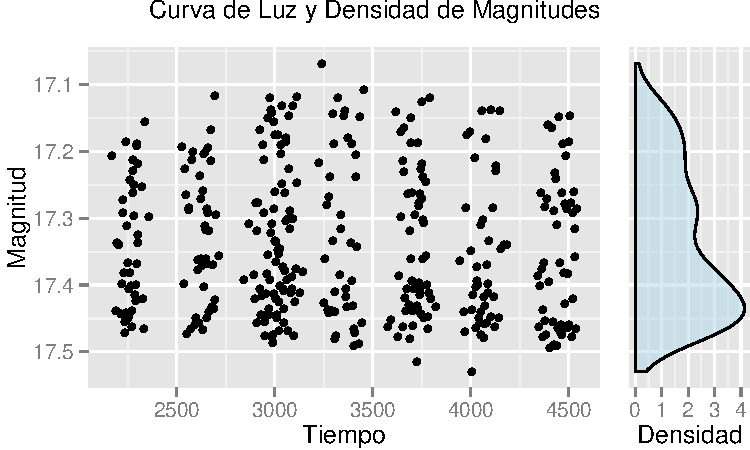
\includegraphics[width = 0.8\textwidth]{./img/CClasificacion/curvaHist.pdf}
  \caption{Curva de luz OGLE-LMC-CEP-0503 y densidad estimada de las magnitudes. }
  \label{fig:curvaHist}
  \centering
\end{figure}

La media $\mu$ y la desviación estándar $\sigma$ (ver cuadro \ref{cuadro:variablesUtilizadas}) son variables descriptivas bien conocidas. En este caso la media es el valor al rededor del cual la serie de magnitudes oscila y la desviación una medida de la amplitud de estas oscilaciones. (Dar argumentos astronómicos). La figura \ref{fig:mediaDesv} muestra la densidad de cada una de las clases en el plano $\mu$-$\sigma$. Aunque las diferentes clases se superponen en este plano, hay pares de clases que pueden ser distinguidas como $\delta$Sct y RRLyr.

\begin{figure}
  \centering
  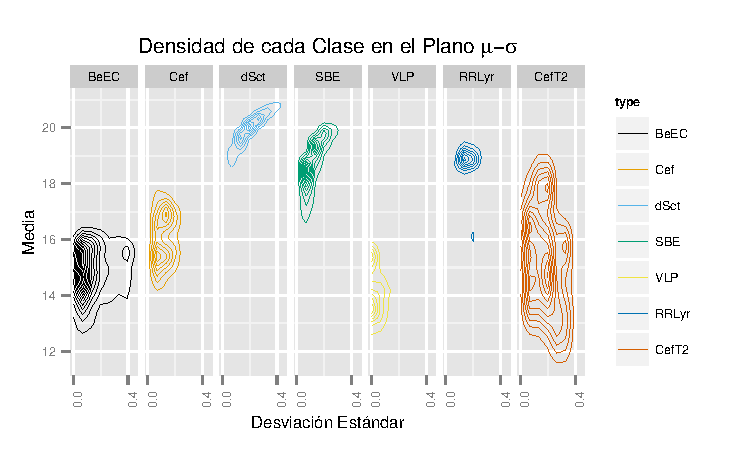
\includegraphics[width = \textwidth]{./img/CClasificacion/mediaDesv.pdf}
  \caption{}
  \label{fig:mediaDesv}
  \centering
\end{figure}

Basado en el trabajo de \cite{rodriguez_feliciano_alisis_2012} utilizamos el sesgo y la curtosis como características. El sesgo es el tercer momento central estandarizado \footnote{El k-ésimo momento centrado de una variable aleatoria $X$ (o de su distribución) es $\mu_{k} =E[(X-\mu)^{k}]$, siendo $\mu$ su media. Su k-ésimo momento central estandarizado es $\frac{\mu_k}{\sigma^k}$, siendo $\sigma$ la desviación estándar.} y es una medida de de la asimetría de una distribución. Una distribución es simétrica si su sesgo es $0$, su cola izquierda es más larga si su sesgo es positivo y su cola derecha es más larga si su sesgo es negativo. Por su parte la curtosis es el cuarto momento central estndarizado. Es una medida de qué tan concentrada está la distribución al rededor de la media. La curtosis de una distribución normal es $3$ y con frecuencia se estudia una cantidad llamada exceso de curtosis que es el resultado de restarle $3$ a la curtosis. Los autores de \cite{rodriguez_feliciano_alisis_2012}  encontraron que algunos tipos de variabilidad estelar podían ser distinguidos utilizando clasificadores lineales en el plano sesgo-curtosis.

Dado que la estimación de el sesgo y la curtosis con las fórmulas del cuadro \label{cuadro:variablesUtilizadas} requiere de calcular las potencias $(\mu-m_i)^3$ y $(\mu-m_i)^4$, son propensas a dar estimaciones erróneas en el caso de que existan datos atípicos. Calculamos también la l-curtosis y el l-sesgo\footnote{Los l-momentos son combinaciones lineales de los estadísticos de orden. Son robustos, toman valores entre 0 y 1, y la interpretación de sus valores es análoga a la de los momentos. De la misma manera en que se define el sesgo y la curtosis muestral, es posible definir la l-curtosis y el l-sesgo. Fuero propuestos en (cita l-momentos) y su cálculo fue realizado utilizando el paquete lmoments(cita paquete l-moments) para R} y reemplazando el sesgo y la curtosis por estas cantidades no encontramos dierencias importantes en el poder para clasificar de los clasificadores que utlizamos. Esto puede ser un indicador de que no existe una proporción grande de datos atípicos en las curvas de luz. Por su simplicidad utilizamos el sesgo y la curtosis.  


\section{Clasificación}
\subsection{K Vecinos Más Cercanos}
\begin{table}[ht]
  \centering
  \caption{k = 1} 
  \label{table:cmknn}
  \begin{tabular}{rrrrrrrr}
    \hline
    & becand & cep & dcst & ebs & lpv & rrlyr & t2cep \\ 
    \hline
    becand & 381 &   1 &   0 &  50 &  41 &   0 &   0 \\ 
    cep &   1 & 6595 &   4 & 172 &  54 & 986 &  87 \\ 
    dcst &   0 &   7 & 2064 & 340 &  13 & 151 &   0 \\ 
    ebs &  51 & 184 & 536 & 30129 & 573 & 668 &  29 \\ 
    lpv &  42 & 187 &  19 & 944 & 342740 & 371 & 158 \\ 
    rrlyr &   0 & 971 & 165 & 595 & 308 & 41911 & 217 \\ 
    t2cep &   0 &  59 &   0 &  29 &  53 & 130 & 112 \\ 
    \hline
  \end{tabular}
\end{table}

\begin{table}[ht]
  \centering
  \caption{k=1, validación cruzada de 10 iteraciones} 
  \label{table:cmCvKnn}
  \begin{tabular}{rrrrrrrr}
    \hline
    & becand & cep & dcst & ebs & lpv & rrlyr & t2cep \\ 
    \hline
    becand & 0.80 & 0.00 & 0.00 & 0.00 & 0.00 & 0.00 & 0.00 \\ 
    cep & 0.00 & 0.82 & 0.00 & 0.01 & 0.00 & 0.02 & 0.14 \\ 
    dcst & 0.00 & 0.00 & 0.74 & 0.01 & 0.00 & 0.00 & 0.00 \\ 
    ebs & 0.11 & 0.02 & 0.19 & 0.93 & 0.00 & 0.02 & 0.05 \\ 
    lpv & 0.09 & 0.02 & 0.01 & 0.03 & 1.00 & 0.01 & 0.26 \\ 
    rrlyr & 0.00 & 0.12 & 0.06 & 0.02 & 0.00 & 0.95 & 0.36 \\ 
    t2cep & 0.00 & 0.01 & 0.00 & 0.00 & 0.00 & 0.00 & 0.19 \\ 
    \hline
  \end{tabular}
\end{table}

\subsection{Árboles de clasificación y regresión}
% Matriz de confusión para Cart
\begin{table}[ht]
  \centering
  \caption{Matriz de confusión para CART} 
  \label{cuadro:cmCart}
  \begin{tabular}{rrrrrrrr}
    \hline
    & becand & cep & dcst & ebs & lpv & rrlyr & t2cep \\ 
    \hline
    becand & 470 &  12 &   6 & 1039 & 8906 &  47 &  18 \\ 
    cep &   0 & 6210 &  12 &  18 & 320 & 3098 &  92 \\ 
    dcst &   0 &  35 & 2511 & 5538 &  91 & 1615 &   1 \\ 
    ebs &   0 &   1 & 148 & 21346 & 346 &  64 &   1 \\ 
    lpv &   5 & 107 &  24 & 1762 & 304810 & 100 &   3 \\ 
    rrlyr &   0 & 648 &  82 & 552 & 13880 & 34313 &  92 \\ 
    t2cep &   0 & 991 &   5 & 2004 & 15429 & 4980 & 396 \\ 
    \hline
  \end{tabular}
\end{table}

% Errores de validación cruzada para cart
\begin{table}[ht]
  \centering
  \caption{Tasas de clasificación estimadas por validación cruzada de 10 iteraciones} 
  \label{table:cmCvart}
  \begin{tabular}{rrrrrrrr}
    \hline
    & becand & cep & dcst & ebs & lpv & rrlyr & t2cep \\ 
    \hline
    becand & 0.99 & 0.00 & 0.00 & 0.03 & 0.03 & 0.00 & 0.03 \\ 
    cep & 0.00 & 0.78 & 0.00 & 0.00 & 0.00 & 0.07 & 0.15 \\ 
    dcst & 0.00 & 0.00 & 0.90 & 0.17 & 0.00 & 0.04 & 0.00 \\ 
    ebs & 0.00 & 0.00 & 0.05 & 0.66 & 0.00 & 0.00 & 0.00 \\ 
    lpv & 0.01 & 0.01 & 0.01 & 0.05 & 0.89 & 0.00 & 0.00 \\ 
    rrlyr & 0.00 & 0.08 & 0.03 & 0.02 & 0.04 & 0.78 & 0.15 \\ 
    t2cep & 0.00 & 0.12 & 0.00 & 0.06 & 0.04 & 0.11 & 0.66 \\ 
    \hline
  \end{tabular}
\end{table}

\subsection{Máquinas de Soporte Vectorial}

\begin{table}[ht]
  \centering
  \caption{$\gamma = 0.1$, costo = $16$} 
  \label{table:cmSvm}
  \begin{tabular}{rrrrrrrr}
    \hline
    & becand & cep & dcst & ebs & lpv & rrlyr & t2cep \\ 
    \hline
    becand & 297 &   0 &   2 &  26 &  16 &   0 &   0 \\ 
    cep &   0 & 4622 &   0 &  55 &  85 & 788 &  69 \\ 
    dcst &   0 &   0 & 1683 & 163 &   4 &  47 &   0 \\ 
    ebs &  89 &  48 & 865 & 29439 & 198 & 563 &   5 \\ 
    lpv &  89 & 490 &  22 & 1380 & 342823 & 1113 & 255 \\ 
    rrlyr &   0 & 2844 & 216 & 1196 & 656 & 41706 & 274 \\ 
    t2cep &   0 &   0 &   0 &   0 &   0 &   0 &   0 \\ 
    \hline
  \end{tabular}
\end{table}

\begin{table}[ht]
  \centering
  \caption{$\gamma = 0.1$, costo = $16$, validación cruzada de 10 iteraciones} 
  \label{table:cmCvSvm}
  \begin{tabular}{rrrrrrrr}
    \hline
    & becand & cep & dcst & ebs & lpv & rrlyr & t2cep \\ 
    \hline
    becand & 0.63 & 0.00 & 0.00 & 0.00 & 0.00 & 0.00 & 0.00 \\ 
    cep & 0.00 & 0.58 & 0.00 & 0.00 & 0.00 & 0.02 & 0.11 \\ 
    dcst & 0.00 & 0.00 & 0.60 & 0.01 & 0.00 & 0.00 & 0.00 \\ 
    ebs & 0.19 & 0.01 & 0.31 & 0.91 & 0.00 & 0.01 & 0.01 \\ 
    lpv & 0.19 & 0.06 & 0.01 & 0.04 & 1.00 & 0.03 & 0.42 \\ 
    rrlyr & 0.00 & 0.36 & 0.08 & 0.04 & 0.00 & 0.94 & 0.45 \\ 
    t2cep & 0.00 & 0.00 & 0.00 & 0.00 & 0.00 & 0.00 & 0.00 \\ 
    \hline
  \end{tabular}
\end{table}

\subsection{Bosques Aleatorios}


% \begin{appendices}

%   \chapter{El Problema de Aprendizaje} %\label{sec:problemaAprendizaje}}

%   \chapter{K Vecinos Más cercanos}

%   \chapter{Árboles de Clasificación y Regresión}

%   \chapter{Máquinas de Soporte Vectorial}
  
%   \chapter{Bosques Aleatorios}
  
% \end{appendices}

%\chapter{Cosas que la evolución se llevó}

%\section{vieja introducción}
% En este trabajo abordamos el problema de clasificar curvas de luz de estrellas variables por su tipo de variabilidad \footnote{Las estrellas variables son estrellas cuya magnitud cambia en el tiempo (ver nota \ref{nota:curvasDeLuz}). Pueden ser periódicas o no periódicas y se pueden clasificar como pulsantes, eruptivas o variables eclipsantes aunque existen subclases de variabilidad estelar. Una estrella puede ser clasificada en estas subclases conociendo su curva de luz (ver el capítulo 13 de \cite{karttunen_fundamental_2007}).} como un problema de aprendizaje supervisado. Para esto utilizamos una parte de los resultados de la tercera fase del \textit{Optical Gravitational Lensing Experiment} (OGLE III) que contiene curvas de luz  de estrellas previamente clasificadas en seis tipos de variabilidad estelar y curvas de luz de estrellas candidatas a ser clasificadas como Be (ver capítulo \ref{cap:losDatos}) (ver cuadro \ref{cuadro:datosUsados}). 


% Para abordar el problema de clasificación adoptamos el siguiente punto de vista. Cada curva de luz $c_i = \{(t_{n}^{i}, m_{n}^{i})\}_{n}$ es una sucesión de parejas donde la primera es el tiempo y la segunda es la magnitud medida en ese instante.  Debido a limitaciones en el tiempo de observación, fallas técnicas, periodos de matenimiento de los instrumentos utilizados y el hecho de que no todas las regiones del cielo son observables durante todo el año y solo se puede observar una región limitada en cada oportunidad, las curvas de luz no constan del mismo número de observaciones y éstas no son hechas en intervalos regulares ($t_{k} - t_{k+1}$ no es constante). Una forma de hacer frente a esto es asignarle a cada curva de luz $c_i$ un vector de atributos $\vec{x_{i}} = \vec{x_{i}}(c_i)\in\mathbb{R}^{n}$ calculados a partir de de $c_i$ (ver sección \ref{sec:atributos}) que intenten describir los tipos de variabilidad. Como los elementos de la muestra han sido clasificados previamente, le asignamos a cada curva de luz $c_i$ una etiqueta $j_i\in J=\{\text{RR Lyr}, \dots, \text{BeSC}\}$ (ver tabla \ref{cuadro:datosUsados}) que corresponde al tipo de variabilidad estelar de la estrella observada.  Dicha etiqueta, a su vez, es heredada por el vector de atributos $\vec{x}_i$.

% Si nuestra elección de atributos es acertada, podremos utilizar la representación de las curvas de luz en el espacio de atributos para realizar la clasificación, esto es, existirá una función $g:\mathbb{R}^n\rightarrow J$ que, de alcanzar la mejor tasa de clasificación correcta posible para esos atributos, le asigna a cada curva de luz el tipo de variabilidad correcto con probabilidad alta (ver capítulo \ref{cap:problemaAprendizaje}). Puede suceder que, si los atributos no caracterizan los diferentes tipos de variabilidad, incluso utilizando el mejor clasificador posible (la mejor función $g$) no sea posible alcanzar errores de clasificación bajos. De esto se sigue que la elección de atributos es crucial para lograr una buena clasificación. La elección de los atributos utilizados se discute en la sección \ref{sec:atributos}.

% El siguiente problema será el de inferir (aprender) de los datos una función $\hat{g}:\mathbb{R}^n\rightarrow J$ que se aproxime tanto como sea posible a la mejor regla posible en cuanto a que maximice la probabilidad de clasificación correcta. Para encontrar esta regla existen diferentes aproximaciones y algorítmos que permiten la división del espacio de atributos en zonas a cada una de las cuales se le asigna un tipo de variabilidad. En la práctica no se conoce la mejor regla posible porque esto requeriría el conocimiento de la distribución exacta de los atributos (ver capítulo \ref{cap:problemaAprendizaje}). Tampoco se conoce el mínimo error de clasificación posible por lo que, para la selección del mejor clasificador entre los posibles, se utilizan estimaciones del error de clasificación que utilizan la muestra disponible, en este caso validación cruzada (ver sección \ref{sec:estimacionError}).En el capítulo \ref{cap:aprendizaje} utilizamos k vecinos más cercanos, arboles de clasificación y regresión; y maquinas de soporte vectorial para inferir la función $\hat{g}$. Asímismo analizamos los estimados de la probabilidad de error al usar cada algorítmo y comentamos las ventajas comparativas de cada uno. Estos tres métodos son muy diferentes en su naturaleza, fueron elegidos porque han mostrado ser efectivos en gran variedad de aplicaciones y por su carácter no paramétrico y no lineal. 

% Así la clasificación de una curva de luz correspondiente a una estrella cuyo tipo de variabilidad es desconocido será un proceso de dos pasos. El primero será la extracción de los atributos. El segundo paso será la clasificación basada en los atributos utilizando la función $\hat{g}$ que fue encontrada con ayuda de la muestra disponible. Esta clasificación será correcta con cierta probabilidad, estimada con validación cruzada.

% Este documento está organizado de la siguiente manera. En el capítulo \ref{cap:losDatos} damos un análisis descriptivo del conjunto de datos que consideramos y discutimos la elección de los atributos para realizar la clasificación. En el capítulo \ref{cap:problemaAprendizaje} discutimos brevemente el problema de clasificación en general, describimos el mejor clasificador posible (el clasificador de Bayes), discutimos la imposibilidad de utilizarlo en la mayoría de aplicaciones complejas y describimos el método que usamos para estimar la probabilidad de error de los clasificadores. En el capítulo \ref{cap:aprendizaje} describimos los métodos de clasificación utilizados, damos los estimados del error de clasificación y comparamos los resultados con otros valores dados en la literatura.

\bibliographystyle{plain}
\bibliography{tesisMatematicas}

\end{document}
